\documentclass{article}
\usepackage[utf8]{inputenc}
\usepackage{listings}

\title{EDA132 Project2 - Probabilistic Reasoning}
\author{Axel Larsson (920515-0395), Lewis Belcher (900429-3552)}
\date{}

\usepackage{natbib}
\usepackage{graphicx}
\usepackage{mathtools}
\usepackage[thinlines]{easytable}
\usepackage{placeins}

\begin{document}

\maketitle

\section{Introduction}
In this project we employ a Hidden Markov Model to do filtering for localisation in an environment with no landmarks.

\subsection{The Environment}
The environment is modelled as an empty room; a rectangular grid of size $n \times{m}$ where $n$ is the number of rows and $m$ the number of columns. The time is seen as integers, we start at time $t = 0$. Each time step corresponds to the robot moving one field in any direction and the sensor giving an approximation of the location of the robot. The true location of the robot is a triple of $(x, y, heading)$ called a pose, e.g. the pose $(0, 1, EAST)$ corresponds to Figure \ref{fig:grid}.

\begin{figure}[ht]
\centering
    \begin{TAB}(e,2cm,2cm){|c:c:c:c|}{|c:c:c|}
    &  $\to$    &   &     \\
    &           &   &     \\
    &           &   &      
    \end{TAB}
\caption{An example grid of size $3 \times{4}$ with the robot's pose $(0,1, EAST).$}
\label{fig:grid}
\end{figure}



\subsection{Robot and Sensors}\label{sec:robots}
The robot moves autonomously in one of the four cardinal directions, denoted $NORTH$, $EAST$, $SOUTH$ and $WEST$ depending on whether or not it encounters a wall. The moving strategy is given in Table \ref{tab:robot}. If the robot encounters a wall it always changes heading and the new heading is chosen from a uniform distribution over the available headings that does not entail wall encounters. Thus, if the robot is in the north west corner there is a $50\%$ probability of the new heading being east and a $50\%$ probability of it being south.
\begin{table}[ht]
\centering
  \begin{tabular}{ | l | l | }
    \hline
    \textbf{Heading}                            & \textbf{Probability}  \\ \hline
    $P(Maintain\ heading \mid no\ wall)$      & $0.7$                 \\ \hline
    $P(Change\ heading \mid no\ wall)$        & $0.3$                 \\ \hline
    $P(Maintain\ heading \mid wall)$          & $0.0$                 \\ \hline
    $P(Change\ heading \mid wall)$            & $1.0$                 \\ \hline
  \end{tabular}
  \caption{The robot's moving strategy, depending on wall encounter.}
  \label{tab:robot}
\end{table}

The objective is to localise and track a robot whose location is hidden. The only data available comes from a noisy sensor that approximates the location of the robot. The sensor reports the location of the robot as a pair of coordinates, $(x, y)$ on the grid. The sensor can report four different types of readings; $L$, $L_s$, $L_{s2}$ and "Nothing". $L$ denotes the correct location, $L_s$ any of the $8$ surrounding fields of the true location $L$ on the grid and $L_{s2}$ the next 16 surrounding fields. Note that this can include locations that are actually outside the grid, e.g. if the robot's true location is a corner field, the sensor might report the location as being $(-1, -1)$. The probability for each type of reading is shown in Table \ref{tab:sensor}.

\begin{table}[ht]
\centering
  \begin{tabular}{ | l | l | }
    \hline
    \textbf{Sensor Reading}             & \textbf{Probability}  \\ \hline
    True location $L$                   & $0.1$                 \\ \hline
    Surrounding fields $L_s$            & $0.05$                \\ \hline
    Next surrounding fields $L_{s2}$    & $0.025$               \\ \hline
    "Nothing"                           & $0.1$                 \\ \hline
  \end{tabular}
  \caption{Probabilities for the different possible sensor readings.}
  \label{tab:sensor}
\end{table}

\subsection{Probabilistic Reasoning}
We construct an agent operating in a partially observable environment. This agent maintains a belief state of which states of the world are currently probable. The agent predicts from the belief state and a transition model how the world might evolve in the next time step. The agent receives percepts from a noisy sensor and updates its belief state with the help of a sensor model.

A transition model specifies the probability distribution over the latest state variables given the previous values. In general we denote this variable $X_t$ where $t$ is the time step. So, $X_0$ would denote the state of the world at $t = 0$. In our world the state variable is the pose of the robot. If we assume a first-order Markov process, i.e. that the current state depends on only the previous state, we can write: 
\begin{displaymath}
\textbf{P}(\textbf{X}_t \mid \textbf{X}_{0:t-1}) = \textbf{P}(\textbf{X}_t \mid \textbf{X}_{t-1})
\end{displaymath} Where $\textbf{X}_t$ are the state variables. Hence, the transition model says that the next state is only dependent on the previous state.
Furthermore we denote the evidence variable as $E_t$ which corresponds to the sensor output of a pair of coordinates $(x, y)$. For the sensor model, we make the \emph{sensor Markov assumption}:
\begin{displaymath}
\textbf{P}(\textbf{E}_t \mid \textbf{X}_{0:t}, \textbf{E}_{0:t-1} = \textbf{P}(\textbf{E}_t \mid \textbf{X}_t)
\end{displaymath} Thus, the state of the world causes the sensors to take on particular values.

Filtering is the process of computing the belief state, the posterior distribution over the most recent state given all evidence to date. To do filtering we compute:
\begin{displaymath}
\textbf{f}_{1:t} = \textbf{P}(\textbf{X}_t \mid \textbf{e}_{1:t})
\end{displaymath}

A \textbf{hidden Markov model}, or \textbf{HMM} is a temporal probabilistic model in which the state of the world is described by a \textbf{single discrete} random variable and whose possible values are the possible states of the world. If we enumerate the different possible states, i.e. the values of $X_t$, with $1,..,S$ the transition model $\textbf{P}(X_t \mid X_{t-1})$ becomes an $S \times S$ matrix $\textbf{T}$. $\textbf{T}_{i,j}$ is the probability of a transition from state $i$ to state $j$ which can be written as 
\begin{displaymath}
\textbf{T}_{i,j} = P(X_t = j \mid X_{t-1} = i)
\end{displaymath}

We also introduce an $S \times S$ diagonal matrix $\textbf{O}_t$ whose $i$:th diagonal entry is $P(e_t \mid X_t = i)$, i.e. we specify how likely it is that the state causes $e_t$ to appear, for each state $i$. The $t$ specifies the time step and thus the current evidence is known at that time.

With a hidden Markov model we can do filtering with the following equation:
\begin{displaymath}
\textbf{f}_{1:t+1} = \alpha \textbf{O}_{t+1} \textbf{T}^t\textbf{f}_{1:t}
\end{displaymath}
where \textbf{f} is a column vector over the belief state; the probability distribution over the most recent state given all evidence to date. The equation is recursive, and we set the initial $\textbf{f}_{1:0}= \textbf{P}(\textbf{X}_0)$ to reflect the fact that at the the start of the process, $t=0$, all states are equally likely since we have not been given any evidence at this time.

\section{Method}
The possible different states are given as poses, i.e. $(x,y,heading)$. They need to be encoded in the transition matrix $\textbf{T}$ so that $\textbf{T}_{i,j}$ gives the probability of the robot transitioning to pose $j$ from pose $i$. We translate a pose to an index $i$ or $j$ by enumerating the headings clockwise from $0$ to $4$ starting with $NORTH$. This is described in Table \ref{tab:headings}.

\begin{table}[ht]
\centering
  \begin{tabular}{ | l | c | }
    \hline
    \textbf{Heading}    & \textbf{Code}   \\ \hline
    $NORTH$             & $0$             \\ \hline
    $EAST$              & $1$             \\ \hline
    $SOUTH$             & $2$             \\ \hline
    $WEST$              & $3$             \\ \hline
  \end{tabular}
  \caption{Encoding the headings.}
  \label{tab:headings}
\end{table}
We then multiply the heading code with $4$ and add the encoding of the location $(x,y)$ as a simply enumeration of the fields as row-major order. Thus we have:
\begin{lstlisting}
pose_to_index(x,y,h) = sq_nbr(x,y) * 4 + heading_code(h)
\end{lstlisting} to compute the index of a certain pose. For instance the pose $(0,1,EAST)$ would be translated to $1*4 + 1 = 5$, which corresponds to the robot pose shown in Figure \ref{fig:grid} and the pose $(0,0,EAST)$ would be equal to $1$. So to find the probability of going from pose (i.e. state) $(0,0,EAST)$ to $(0,1,EAST)$ we look up the transition matrix cell $\textbf{T}_{1, 5}$ which should be equal to $0.7$ according to Table \ref{tab:headings}.

The observation matrix is constructed as a diagonal matrix with the probabilities of the robot location on each diagonal element. In this project we receive only the robot location from the sensor, so where we have four states for each position in our transition matrix (as described above) we have four consecutive (along the diagonal) and equal probabilities for each position in the observation matrix.


\section{Implementation}
The program is written in Python3 and the functionality is divided into different modules, located in the \texttt{robot\_localisation} package:
\begin{itemize}
    \item \texttt{grid.py}
    \item \texttt{hmm\_filter.py}
    \item \texttt{main.py}
    \item \texttt{robot.py}
\end{itemize}
The \texttt{main} module is where the CLI is set up and where the robot simulation and tracking is initialised. This module also computes the error between the belief state and the actual state in the form of the so called Manhattan distance.

The \texttt{robot} module contains the logic for the simulation of the robot movement as well as the \texttt{Sensor} class. The \texttt{Sensor} generates readings with the help of numpy according to the distribution explained in Section \ref{sec:robots}. The \texttt{Sensor} class is also responsible for generating the observation matrices depending on the current sensor reading. 

The \texttt{hmm\_filter} module contains a class, \texttt{FilterState}, that does the filtering.
In the \texttt{grid} module, the transition matrix is computed and the representation of the environment (i.e. the grid) is stored. 

\subsection{Usage}
The program root is to be found at \texttt{/h/d5/f/dat11al1/robot-localisation}, while standing in that directory, execute \texttt{python3 robot\_localisation -h} to get a useful help message as such:
\begin{lstlisting}
usage: robot_localisation [-h] [-r ROWS] [-c COLUMNS]

Robot localisation with HMM

optional arguments:
  -h, --help                     show this help message
                                 and exit
  -r ROWS, --rows ROWS           the number of rows on
                                 the grid, default is 4
  -c COLUMNS, --columns COLUMNS  the number of columns on
                                 the grid, default is 4
\end{lstlisting}
As can be seen above, the \texttt{--rows} and \texttt{--cols} command line arguments are used to specify the desired grid size.

\subsection{Requirements}
The minimum requirements to execute the program is:

\begin{itemize}
    \item Python3
    \item numpy
\end{itemize}
If \texttt{virtualenv}, \texttt{setuptools} and \texttt{pip} is available on the system (which, unfortunately, they are not on the student computer system), these can be used to install the program in a virtual environment, but this is entirely optional.

\subsection{Running the Program}
While standing in the project root (\texttt{/h/d5/f/dat11al1/robot-localisation}) with a terminal, execute the command \texttt{python3 robot\_localisation}.

The program is developed as a CLI - Command Line Interface. Upon execution, the program outputs a friendly help text of how to run it, this message can at any time be displayed by typing \texttt{help}. The simulation starts at $t = 0$ and to step forward, one simply presses enter on the keyboard.

The transition and observation matrices can at any time be displayed by invoking \texttt{show T} and \texttt{show O}, respectively. Similarly the column vector representing the belief state of the agent can be shown by \texttt{show f}.

To quit, enter \texttt{q}.

\subsection{Testing}

There are three test modules; \texttt{grid\_test}, \texttt{manhattan\_text} and \texttt{robot\_test}, all located in the \texttt{tests} directory. To execute any of them, go to the project root (\texttt{/h/d5/f/dat11al1/robot-localisation}) and type the command: \texttt{python3 tests/<test-module>.py}.
 
 
\section{Results}

Figures \ref{fig:manhattan-errors} and \ref{fig:manhattan-errors-single} show the errors (Manhattan distance from the true location to the inferred location) compared to the number of steps taken in the simulation, over an average of 20 simulations and for a single simulation respectively.

\begin{figure}[h!]
    \centering
    \textbf{Manhattan distance between true position and \\ inferred position}
    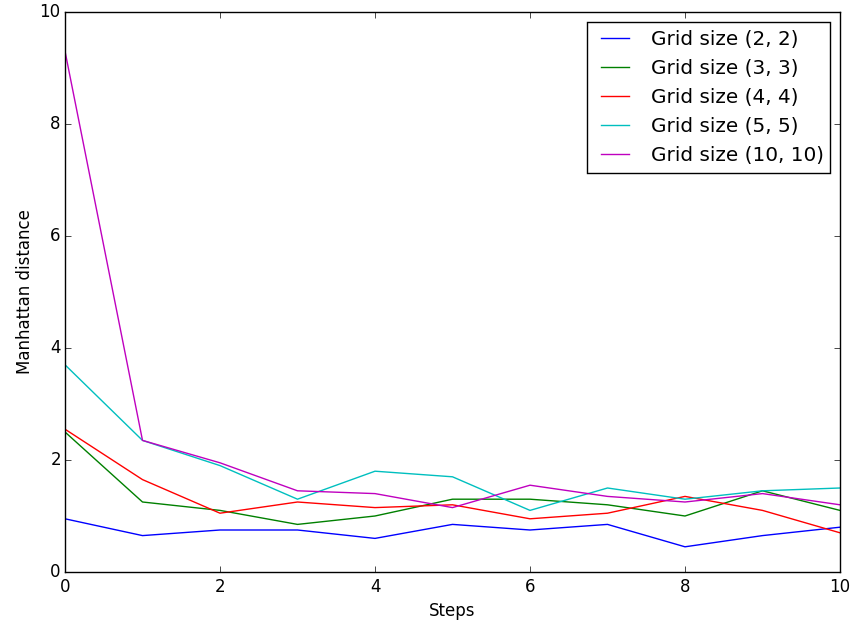
\includegraphics[scale=0.45]{manhattan-errors-notitle.png}
    \caption{The average Manhattan distance between the true robot location and the assumed location using hidden Markov model filtering. The distances were taken over an average of 20 simulations.}
    \label{fig:manhattan-errors}
\end{figure}

\begin{figure}[h!]
    \centering
    \textbf{Manhattan distance between true position and \\ inferred position for a single simulation}
    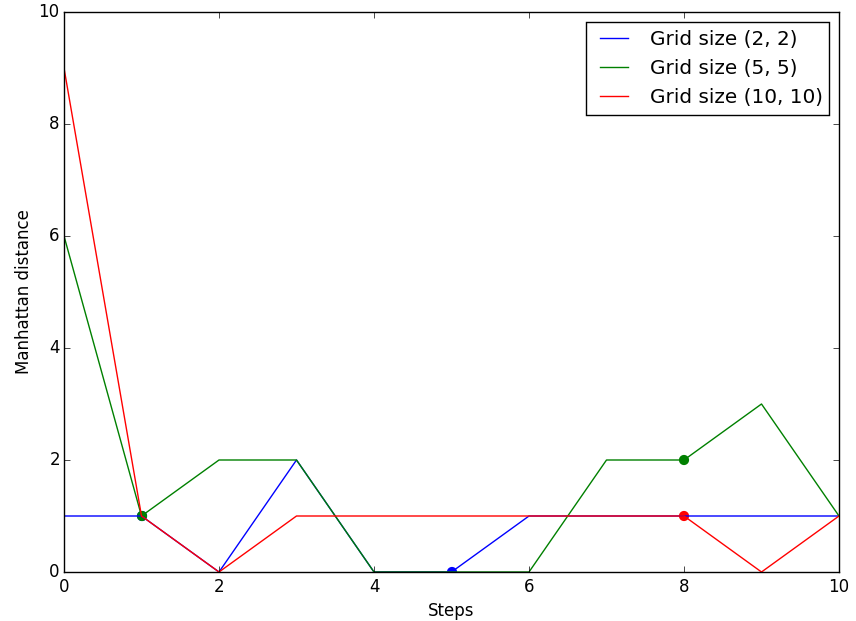
\includegraphics[scale=0.45]{manhattan-errors-single.png}
    \caption{Manhattan distance between the true robot location and the assumed location using hidden Markov model filtering. This plot is for a single simulation and points at which the sensor returned no reading were recorded and plotted as dots in the figure.}
    \label{fig:manhattan-errors-single}
\end{figure}



\FloatBarrier
\section{Discussion}

We find that during the execution of our code the FilterState class finds the location of the robot at an error of 1-2 Manhattan distance within 1-2 steps. For continued execution of the code the belief state is rarely greater than 2 Manhattan distance away. Figure \ref{fig:manhattan-errors} exemplifies this, we see that over an average of 20 simulations for different grid sizes the error converges to a Manhattan distance of between 1-2 at greater than 2 steps.

We also note that one of the primary causes of an incerasing error is when the sensor returns no value (shown in figure \ref{fig:manhattan-errors-single}). In our implementation we do not update our position for these cases, so this result is in line with intuition (only the robot position is changed, and unless it moves directly towards our estimated position the error will increase).

When the sensor gives positions that are outside the grid, we still include them in the calculation. This is something we believe is better than treating off-grid positions as "None". If we treated them as "None", the sensor reading at that time would not give the model any useful information at all. While in our implementation, off-grid positions are not treated any differently than ordinary sensor readings. In the cases where the sensor reports the location as being two steps outside the grid, there could in fact sometimes only be one possible true location that could have caused that sensor reading.
So even if the sensor reports a location that is guaranteed to be incorrect, it still gives the model useful information.

\bibliographystyle{plain}
\bibliography{references}
\end{document}
